
% Header reference level
\clearpairofpagestyles
\chead{\headmark}
\automark[section]{section}
\ifoot{\ifootertext}
\ofoot{\ofootertext}
\cfoot{\thepage}

\section{Taxonomies}
\label{sec:Taxonomies}

This section provides an overview of the taxonomies for the categorization of components, parts thereof, or annotation schemes including (but not limited to) the ones referred to from the coding guidelines in \cref{sec:CodingGuidelines}. The overview is largely summarizing, with essential specification of labels, but limited conceptual elaboration, which is provided in the corresponding guidelines (\cref{sec:CodingGuidelines}). The taxonomies further specify the \begin{emp}label prefixes\end{emp} used to ensure unambiguous reference to the respective taxonomy/ies. Where only the circumstances taxonomy is used, the use of labels is optional.

The extension of existing taxonomies and introduction of additional taxonomies to draw seek epistemological linkage to the field of concern (e.g., to accommodate domain-specific characteristics or analytical necessities) is explicitly permitted. This includes the use of ontologies to support conceptually richer classification of entities. Any adjustment should be clearly indicated as part of the dataset specification (see \cref{sec:Checklist}). 

\begin{emp}Note that the taxonomies in this section are subject to ongoing empirical evaluation and may experience refinement in the future.\end{emp}

\subsection{Context Taxonomy}
\label{subsec:ContextTaxonomy}

The Context Taxonomy captures contextual characterizations with respect to temporal, spatial and various further descriptors that capture institutional context more accurately. It is a systematic extension of the descriptors of the \begin{emp}Conditions\end{emp} component as highlighted in the original grammar specification~\citep{Brady2018InstitutionalGuidelines}. Note that the listed categories include an embedded hierarchy, with more specific labels indented. 

\sp 

\noindent \udl{Specific considerations:}

\begin{itemize}
\item Where possible (and analytically useful/specified in project-specific guidelines), the most specific annotation of a given category should be used (e.g., `point in time', as opposed the more general `temporal' category).
\item Note that selected categories are more general in nature (e.g., the `state' category, since it potentially captures temporal, spatial and domain characterizations). As before, the coder should attempt to classify context in more specific terms.
\item Multiple annotations are explicitly suggested in cases where the characterizations overlap for an annotated element (e.g., `temporal' and `event'). Where possible, the coder may further consider the separation of distinctive activation conditions/execution constraints by category and annotate those correspondingly.
\end{itemize}

\noindent The suggested annotation label prefix -- if applied -- is \begin{emp}\ctx\end{emp}.

\sp

\noindent \udl{Categories:}

\begin{itemize}
\item[] Substantive Context

\begin{itemize}
\item Temporal (tmp) -- Conditions/Constraints associated with time - the when
	\begin{itemize}
	\item Point in time (tim) -- References to specific points in time
		\begin{itemize}
		\item Beginning (e.g., ``from 1st January'')
		\item End (e.g., ``until 31st January'')
		\end{itemize}	
	\item Time frame (tfr) -- References to time frames
	\item Frequency (frq) -- References to frequencies (e.g., ``annually'') 
	\end{itemize}
\item Spatial (spt) -- Conditions/Constraints associated with spatial representations -- the where
	\begin{itemize}
	\item Location (loc) -- References to specific locations
		\begin{itemize}
		\item Beginning
		\item End
		\end{itemize}
	\item Direction (dir) -- References to directions, inclusion of intermediary locations (e.g., ``via'')
	\item Path (pth) -- References to pathways (e.g., ``through the valley'')
	\end{itemize}
\item Domanial (dom) -- Conditions/Constraints applying to a specified activity, topical or existential realm. 
\begin{itemize}
\item Activity realm  (e.g., ``during decision-making'')
\item Topical realm (e.g., ``for drinking water'')
\item Existential realm (e.g., ``during childhood'')
\end{itemize}
\end{itemize}
\end{itemize}

\begin{itemize}
\item[] Procedural Context

\begin{itemize}
\item Order (prc) -- Conditions/Constraints associated with explicit or implied execution (procedural) order (e.g., ``\dots according to the following stages: \dots''). Operationally, this can include expressions of input into the activity identified in the institutional statement (e.g., ``with input from \dots''). Procedural order can further include the explicit specification of required actions at any step in the procedural execution. %, de/activation of other statements or compliance with or violations of statements, respectively.

\item Method (met) -- Conditions/Constraints associated with means or method by which an action is performed, recognizing the following specializations:
	\begin{itemize}
	\item Means -- Action as method (e.g., ``by handshake'')
	\item Instrument -- Artifact as method (e.g., ``by car'')
	\end{itemize}
Note that the method specification is more general than the characterization of distinctive procedural steps under the Procedural `Order' category.
\end{itemize}
\end{itemize}

\begin{itemize}
\item[] Aspirational Context

\begin{itemize}
\item Purpose/Function (pur) -- Conditions/Constraints describing the purpose or intent of an aim or constitutive function; generally output of action (e.g., ``for the purpose of reducing pollution levels'')
%\item Effect -- References to the effect of a given statement on the institutional setting. In contrast to the Purpose characterization, specific emphasis lies on the actual effect, as opposed the underlying intent. This characterization specifically applies to constitutive statements that report a secondary effect affecting the wider institutional setting, besides the immediate effect related to the constituted entity (e.g., its establishment).
\end{itemize}
\end{itemize}

\begin{itemize}
\item[] Situational Context

\begin{itemize}
\item State (ste) -- References to a specific state environmental state (e.g., ``when traffic light is red''); note that state characterization is general in kind and commonly associated with an entity that holds the referenced state (e.g., traffic light).  Where possible, a more specific annotation should be chosen.

%\item State transition (tra) -- Conditions/Constraints referencing a change in state (e.g., ``when the traffic light switches from red to green'')

\item Event (evt) -- Conditions/Constraints referencing specific events (e.g., ``on arrival at the airport \dots''). In contrast to the state characterization, an events is instantaneous in nature, whereas a state can persist over longer time frames and is associated with an entity whose state is described.

\end{itemize}
\end{itemize}

%\item Cause/Reason (cau) -- Conditions/Constraints referencing causes, reasons or justifications for the activation of particular aims or constitutive functions that exist outside the control of the governed action situation, i.e., are exogenous to the action situation. Where such cause is internal to the action situation, consider the `Outcome/Effect' category.

%\item Outcome/Effect (eff) -- Conditions/Constraints describing the outcome or effect of an aim by an actor involved in the action situation -- a change in the environment emanating from the observed actor(s); observation of compliance/non-compliance (e.g., ``if an non-compliant action is observed''; ``if participant fails to meet certification requirements''). This characterization is commonly invoked when coding discretionary actions of observers (e.g., beliefs, suspicions, evaluations), in contrast to exogenous events captured in the `Cause' category.

\newpage

\subsection{Animacy Taxonomy}

The Animacy Taxonomy captures differentiates between animate and inanimate entities, maintaining compatibility with annotation conventions commonly adopted in datasets coded according to the previous IG coding guidelines. The suggested annotation label prefix is \begin{emp}\anim\end{emp}.

\begin{itemize}
\item Animate -- Living entities
\item Inanimate -- Non-living entities, both real and mental constructs
\end{itemize}

\subsection{Metatype Taxonomy}

The Metatype Taxonomy differentiates between concrete physical and abstract entities, e.g., mental constructs. This also applies to component-level nesting (see \cref{subsec:ComponentLevelNesting}) for cases in which an institutional statement is nested in a statement component, such as an object, in which case the object is characterized as abstract in nature. The suggested annotation label prefix is \begin{emp}\metatype\end{emp}.

\begin{itemize}
\item Abstract -- Abstract entities 
\item Concrete -- Concrete entities
\end{itemize}

\subsection{Role Taxonomy}

The role taxonomy serves the annotation of attributes and objects with additional labels to capture their role within a statement structure with respect to the action, organized by relevant role of actor and effect in terms of affected subjects. The suggested annotation label prefix is \begin{emp}\role\end{emp}.

\begin{itemize}
\item Role Characterizations
\begin{itemize}
    \item Originator/Causer/Agent -- Entity from which action originates
    \item Recipient -- Recipient of an artifact/sanction
    \item Possessor -- Owner of an object/entity (e.g., ``house owner'')
\end{itemize}
\item Effect Characterizations
\begin{itemize}
    \item Experiencer -- Indirectly affected actor (e.g., ``observer of non-compliance'')
    \item Advantaged -- Beneficiary distinctively advantaged by referenced activity/function; may not necessarily be recipient (e.g., ``welfare recipient'')
    \item Disadvantaged -- Maleficiary distinctively burdened by referenced activity/function; may not necessarily be recipient
\end{itemize}
%\item Position -- organisation or institutional role assumed by involved actor
\end{itemize}

\subsection{Regulative Functions Taxonomy}
\label{subsec:regfunc}

Some types of syntactic annotations can aid the coder in discerning and capturing information that signals the broader function of institutional statements, as indicated by components of which they are comprised. Those are referred to as ``institutional function'', and more specifically ``regulative functions'' in as far as regulative statements are concerned (Constitutive functions are discussed in \cref{subsec:confunc}). Regulative functions facilitate the annotation of aims in order to capture the correspondence of aims to analytical functions of relevance through specific theoretical lenses. Exemplifying the use of the institutional grammar for the analysis from a regulatory compliance perspective, compliance and violation behaviour is of specific concern, whereas institutional life cycles may require the annotation of action verbs signalling the initiation of termination of institutional arrangements. Note that the offered taxonomy provides examples for regulative functions organized by categories (alongside potential specializations), but does not claim exhaustiveness. The suggested annotation label prefix is \begin{emp}\regfunc\end{emp}.

\begin{itemize}
\item Compliance action -- action reflecting compliance behavior
	\begin{itemize}
	\item Comply -- action reflecting compliance
	\item Violate -- action reflecting violation
	\end{itemize}

\item Monitor -- action reflecting the institutional function of monitoring
	\begin{itemize}
	\item Detect compliance -- action reflecting the detection of compliance
	\item Detect violation -- action reflecting the detection of violation
	\end{itemize}

\item Enforce -- action reflecting enforcement acts
	\begin{itemize}
	\item Reward -- action reflecting rewarding behaviour (regulative-incentivizing)
	\item Sanction -- action reflecting sanctioning behaviour (regulative-punitive)
	\end{itemize}

\item Enforcement response -- action reflecting responses to enforcement outcomes
	\begin{itemize}
	\item Accept -- action reflecting acceptance of enforcement outcome
	\item Reject -- action reflecting rejection of enforcement outcome
		\begin{itemize}
		\item Appeal (specialization of reject) -- action reflecting appeal against enforcement outcome
		\end{itemize}
	\end{itemize}

%\item Process -- Life cycle
%	\begin{itemize}
%	\item Initiate
%	\item Interrupt
%	\item Resume
%	\item Conclude
%	\end{itemize}
%
%\item Transaction -- action reflecting a request and corresponding response
%	\begin{itemize}
%	\item Request -- action reflecting a request.
%	\item Response -- action reflecting a response to a request. Central difference to enforcement responses is lack of a regulatory compliance function.
%		\begin{itemize}
%		\item Accept
%		\item Reject
%		\end{itemize}
%	\end{itemize}
%
%\item Decide -- action reflecting a decision/discretion
%
%\item Inform -- action reflecting information dissemination
%
%\item Declare -- action reflecting change in role, position, environment, institutional fact
%
%\item Assign -- action reflecting the assignment of responsibilities to other actors
%	\begin{itemize}
%	\item Delegate -- action reflecting the delegation of functions/tasks, generally downwards in an organisational structure (e.g., delegation to subordinate)
%	\item Elevate -- action reflecting the elevation of functions/tasks, generally upwards in an organizational structure (e.g., elevation to supervisor)
%	\end{itemize}
\end{itemize}

As noted above, the regulative functions concept is intended to draw the epistemological linkage to analytical frameworks and/or concepts associated with a given domain. 

\subsection{Constitutive Functions Taxonomy}
\label{subsec:confunc}

The constitutive function taxonomy is complementary to the regulative functions taxonomy under the shared  institutional functions umbrella. Constitutive function annotations offer a semantic characterization of specific constitutive functions in relation to the constituted entity and/or the linkage of constituted entity and constituting properties, respectively. The top-level distinction of constitutive functions is the identification of the constituted entity as either an \begin{emp}entity\end{emp} established, modified or otherwise referenced in the context of the policy document, or the \begin{emp}policy\end{emp} itself. On a more fine-grained level, the categories capture the role of the constituting function with respect to the constituted entity (i.e., a specific entity, or the policy). The suggested annotation label prefix is \begin{emp}\confunc\end{emp}.

The structure, alongside specific annotations, is visualized in \cref{fig:ConstitutiveFunctions} and described in the following. 
%
\begin{figure}[h!]
    \centering
    \framedfigure{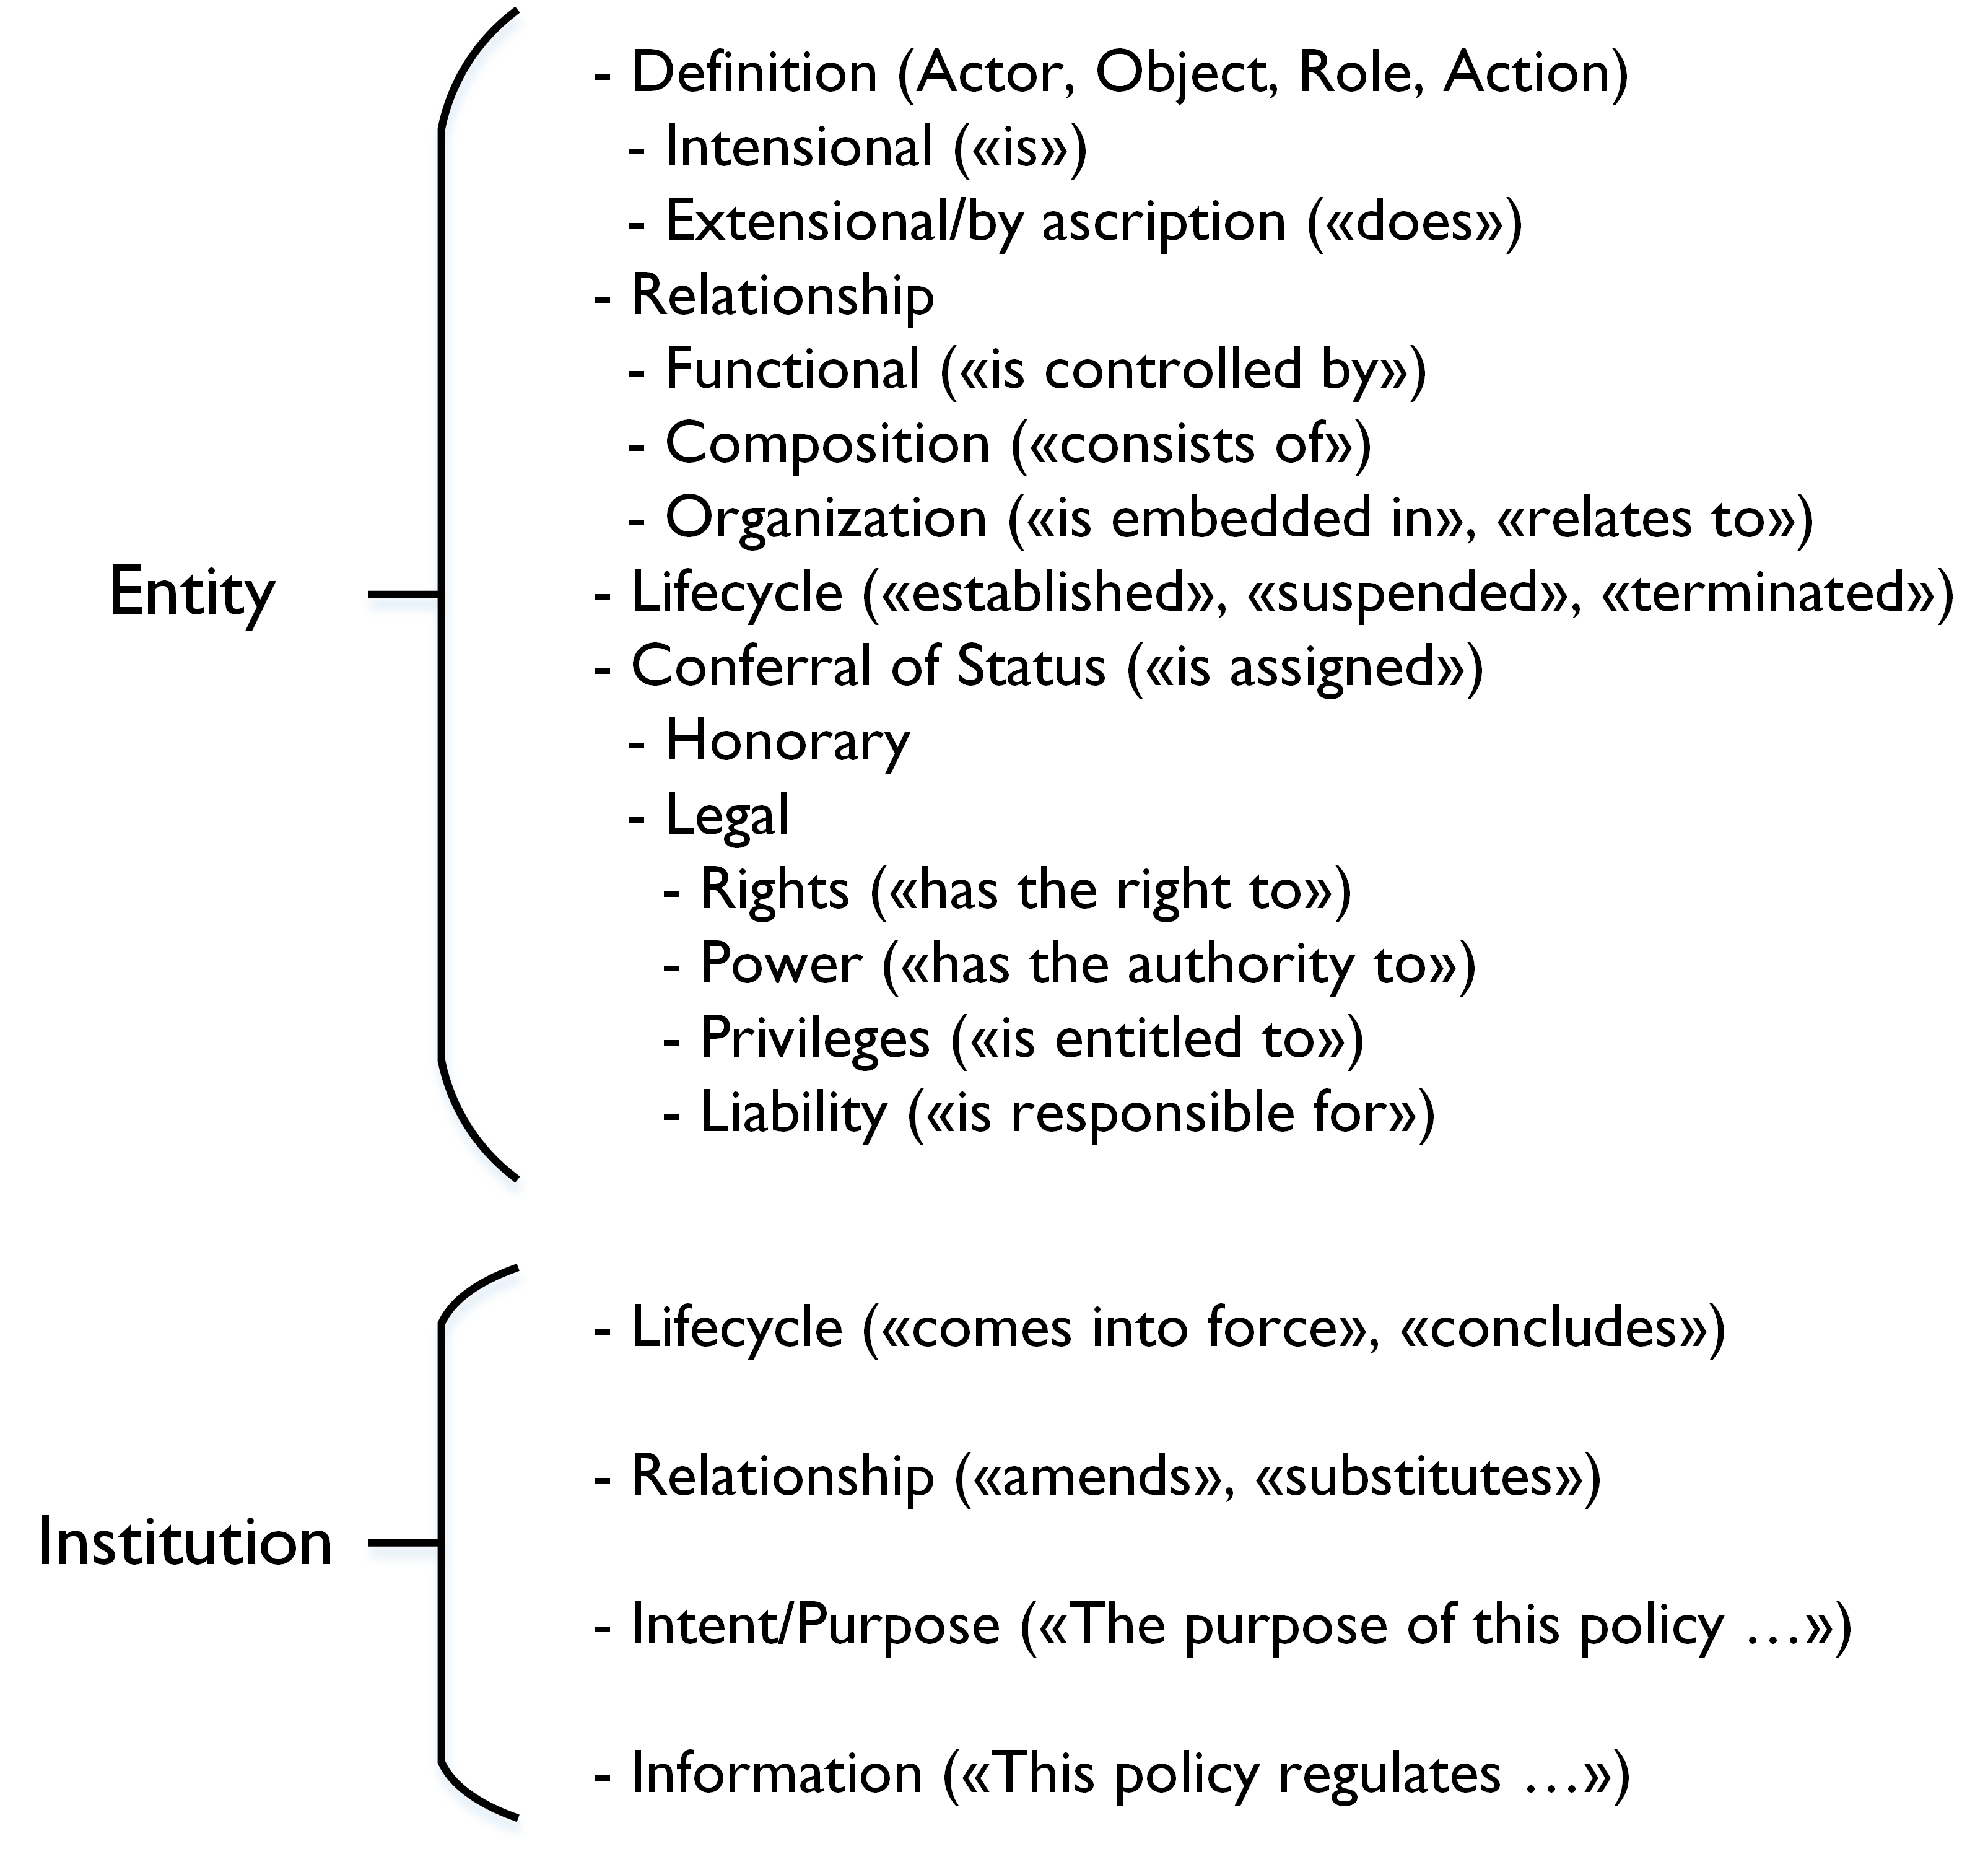
\includegraphics[width=0.75\textwidth]{figures/ConstitutiveFunctions.png}}
    \caption{Constitutive Functions}
    \label{fig:ConstitutiveFunctions}
\end{figure}
%
Where entities are subject to the statement, constitutive functions can capture the definition of constituted entities as relevant for the parameterization of the institutional setting, including actors, object/artifacts, role specifications or actions, alongside status characterizations. This definition is often signaled intensionally (i.e., by explicit definition), or implied by ascription (e.g., implicit characterization of entity based on exhibited behavior, etc.).

In addition to the definition of entities, constitutive functions can capture relationships of different kinds, including organizational relationships in the form of compositions (e.g,. specification of committee membership) and further reflect hierarchical relationships (e.g., leadership structures, embedding positions within organizations).

Possible constitutive functions further include the initiation and termination of entity lifecycles (e.g., dates of appointment termination, etc.). 

Finally, the explicit conferral of status (e.g., in the form of institutional power, such as authority or  competence; rights; privileges, or liability) is a central application of constitutive statements. 

Complementing the perspective on entity specification as part of constitutive statements, constitutive functions that characterize the policy or document itself, have a varying set of functions. Typical characterizations include the policy lifecycle (e.g., date of enactment), as well as its relationship to other policy (e.g., amending or superseding it). Further statements refer to the purpose or intent underlying a given policy. Informational statements offer supplementary information about the document, or state institutional facts contextualizing the policy or domain of concern. Note that the latter is often expressed in terms of statement of fact, rather than institutional statements. 

As with the preceding taxonomies, the constitutive functions taxonomy is subject to further refinement based on ongoing empirical validation efforts.

\section{Statement-Level Annotations}

In addition to annotations pertaining to individual components or component types, annotations may also apply to statements as whole. Most notably, this includes the characterization of statements based on their function in the context of an interlinked institutional statement.

\subsection{Governance Types (Vertical Nesting Annotations)}

The governance annotation relates to the nature of the statement as either \begin{emp}monitored\end{emp} or \begin{emp}consequential\end{emp} to signal regulated, or monitored part of a statement (e.g., \begin{emp}
``citizen must comply with the law, \dots''\end{emp}), in contrast to the consequential statement that signals the associated consequence (e.g., \begin{emp}
``\dots~or else official must sanction citizen.''\end{emp}). Augmenting this, a \begin{emp}monitoring\end{emp} statement highlights the potentially dissociated function of a third-party observer (e.g., bystander, appointed monitor), who may or may not be the enforcer. As a consequence, statements can have multiple statement-level annotations. 

\subsection{Consequence Types}

A second annotation relates to the nature of potential consequences. The main differentiation includes consequences of \begin{emp}existential\end{emp}, and \begin{emp}non-existential\end{emp} kind. 

Consequences of the first kind are understood as ontologically existential, i.e., reflecting whether an entity does not come about, is invalidated, etc. This can further include the institution itself (e.g., lacking preconditions for its continuation), hence leveraging \begin{emp}configurational consequences\end{emp}. 

\begin{emp}Social consequences\end{emp}, as common institutional consequences, are related to economic situation, status, or penalties. As far as the institution is concerned, these are considered non-existential. 

As with other taxonomies, the analyst may introduce subdifferentiations that respond to specific analytical objectives, or establish epistemological linkages to the domain of concern.

The listing of taxonomies complements and concludes the supplementary coding guidelines for the Institutional Grammar 2.0.

%\newpage
